\documentclass[11pt]{article}

% Mandatory Packages
\usepackage{amsmath}
\usepackage{amssymb}
\usepackage{amsthm}
\usepackage{geometry}
\usepackage{tikz}
\usetikzlibrary{arrows.meta, positioning, shapes, patterns}
\usepackage{mathrsfs}
\usepackage{mathtools}
\usepackage{hyperref}

% Page Geometry
\geometry{letterpaper, margin=1in}

% Theorem Environments
\newtheorem{theorem}{Theorem}[section]
\newtheorem{lemma}[theorem]{Lemma}
\newtheorem{proposition}[theorem]{Proposition}
\newtheorem{corollary}[theorem]{Corollary}
\newtheorem{definition}[theorem]{Definition}
\newtheorem{problem}{Problem}
\newtheorem{flawprob}{Diagnostic Problem}

% Custom Commands
\newcommand{\R}{\mathbb{R}}
\newcommand{\N}{\mathbb{N}}
\newcommand{\Z}{\mathbb{Z}}
\newcommand{\Q}{\mathbb{Q}}
\newcommand{\powerset}{\mathcal{P}}

\title{Homework 4: Proofs Involving Cartesian Products of Sets}
\author{Tashfeen Omran}
\date{September 2026}

\begin{document}

\maketitle
\tableofcontents
\newpage

% ==========================================
% PART 1: Comprehensive Introduction
% ==========================================
\section{Part 1: Comprehensive Introduction, Context, and Prerequisites}

\subsection{Core Concepts \& Axioms}
The study of \textbf{Cartesian Products} is a foundational leap in set theory, allowing us to construct higher-dimensional spaces and complex relational structures from simpler, one-dimensional sets. 

\begin{definition}[Ordered Pair]
An ordered pair $(a, b)$ is a collection of two elements where the order matters. Formally, using the Kuratowski definition, $(a, b) = \{\{a\}, \{a, b\}\}$. Two ordered pairs $(a, b)$ and $(c, d)$ are equal if and only if $a = c$ and $b = d$.
\end{definition}

\begin{definition}[Cartesian Product]
For any two sets $A$ and $B$, the Cartesian product $A \times B$ is the set of all ordered pairs $(a, b)$ such that $a \in A$ and $b \in B$. Symbolically:
\[ A \times B = \{ (a, b) \mid a \in A \text{ and } b \in B \} \]
\end{definition}

If either $A = \emptyset$ or $B = \emptyset$, then no such ordered pairs can be formed, and thus $A \times B = \emptyset$.

\subsection{Intuition and Set-Theoretic Foundations}
Imagine $A$ as the set of all possible states of a system, and $B$ as the set of all possible actions an agent can take. The Cartesian product $A \times B$ represents the \textit{state-action space}—every conceivable combination of a state and an action. 

Geometrically, if $A$ is a segment on the x-axis and $B$ is a segment on the y-axis, $A \times B$ forms a rectangular region in the 2D plane. When we perform set operations (union, intersection, difference) on Cartesian products, we are manipulating these multi-dimensional regions. The logic of these manipulations relies heavily on the logical operators AND ($\land$) and OR ($\lor$). Because intersection ($\cap$) maps to AND, and union ($\cup$) maps to OR, the distributive properties of logic directly dictate the distributive properties of Cartesian products.

\subsection{Historical Context and Motivation}
The Cartesian product is named after René Descartes, whose formulation of analytic geometry in the 17th century bridged algebra and Euclidean geometry. By representing points in a plane as pairs of real numbers $(x, y) \in \R \times \R$, Descartes created the coordinate system. In the late 19th and early 20th centuries, mathematicians like Georg Cantor, Ernst Zermelo, and Abraham Fraenkel formalized set theory, recognizing that the Cartesian product was not just a geometric tool, but a fundamental axiom-derived operation necessary for defining relations, functions, and cardinality.

\subsection{Key Theorems, Lemmas, and Formulas}
\begin{theorem}[Distributivity over Union]
For any sets $A, B,$ and $C$:
\[ A \times (B \cup C) = (A \times B) \cup (A \times C) \]
\end{theorem}

\begin{theorem}[Distributivity over Intersection]
For any sets $A, B,$ and $C$:
\[ A \times (B \cap C) = (A \times B) \cap (A \times C) \]
\end{theorem}

\begin{theorem}[Distributivity over Set Difference]
For any sets $A, B,$ and $C$:
\[ A \times (B \setminus C) = (A \times B) \setminus (A \times C) \]
\end{theorem}

\begin{theorem}[Intersection of Products]
For any sets $A, B, C,$ and $D$:
\[ (A \times B) \cap (C \times D) = (A \cap C) \times (B \cap D) \]
\end{theorem}

\subsection{Prerequisites}
To master this chapter, one must be proficient in:
\begin{itemize}
    \item \textbf{Basic Set Theory:} Definitions of $\cup, \cap, \setminus, \subseteq$, and the Power Set $\powerset(A)$.
    \item \textbf{Propositional Logic:} De Morgan's Laws, logical equivalence, and the definitions of conditional ($\implies$) and biconditional ($\iff$) statements.
    \item \textbf{Proof Techniques:} Element-chasing (Direct Proof), Proof by Contrapositive, and handling vacuous truths (empty sets).
\end{itemize}

% ==========================================
% PART 2: Detailed Homework Solutions
% ==========================================
\section{Part 2: Detailed Homework Solutions (Rigorous Proofs \& Computations)}

\textit{Note: In accordance with strategic problem selection, the following problems have been chosen to cover every distinct problem archetype (Power Sets, Empty Sets, Set Equality, Subset Inclusion, and Counterexamples) from Section 4.6.}

\begin{problem}[Exercise 4.61]
For $A = \{1\}$ and $B = \{2\}$, determine $\powerset(A \times B)$ and $\powerset(A) \times \powerset(B)$.
\end{problem}
\begin{proof}[Computation]
First, we determine the Cartesian product $A \times B$:
\[ A \times B = \{(1, 2)\} \]
The power set of a set $S$, denoted $\powerset(S)$, is the set of all subsets of $S$. Since $A \times B$ contains exactly one element, its power set will contain $2^1 = 2$ elements:
\[ \powerset(A \times B) = \{\emptyset, \{(1, 2)\}\} \]

Next, we determine the power sets of $A$ and $B$ individually:
\[ \powerset(A) = \{\emptyset, \{1\}\} \]
\[ \powerset(B) = \{\emptyset, \{2\}\} \]
Now, we compute the Cartesian product of these two power sets, $\powerset(A) \times \powerset(B)$. This is the set of all ordered pairs where the first element is a subset of $A$ and the second element is a subset of $B$:
\[ \powerset(A) \times \powerset(B) = \{ (\emptyset, \emptyset), (\emptyset, \{2\}), (\{1\}, \emptyset), (\{1\}, \{2\}) \} \]
\textit{Final Answer:} $\powerset(A \times B) = \{\emptyset, \{(1, 2)\}\}$ and $\powerset(A) \times \powerset(B) = \{ (\emptyset, \emptyset), (\emptyset, \{2\}), (\{1\}, \emptyset), (\{1\}, \{2\}) \}$.
\end{proof}

\begin{problem}[Exercise 4.62]
Let $A$ and $B$ be sets. Prove that $A \times B = \emptyset$ if and only if $A = \emptyset$ or $B = \emptyset$.
\end{problem}
\begin{proof}[Proof by Contrapositive and Direct Proof]
We must prove a biconditional statement $P \iff Q$. We will prove $P \implies Q$ by contrapositive, and $Q \implies P$ directly.

\textbf{Part 1: Prove $A \times B = \emptyset \implies A = \emptyset \lor B = \emptyset$.}
We proceed by contrapositive. The negation of $A = \emptyset \lor B = \emptyset$ is $A \neq \emptyset \land B \neq \emptyset$ (by De Morgan's Law). The negation of $A \times B = \emptyset$ is $A \times B \neq \emptyset$.
Assume $A \neq \emptyset$ and $B \neq \emptyset$. 
By definition of a non-empty set, there exists at least one element $a \in A$ and at least one element $b \in B$. 
By the definition of the Cartesian product, the ordered pair $(a, b)$ must be an element of $A \times B$. 
Since $A \times B$ contains at least the element $(a, b)$, it follows that $A \times B \neq \emptyset$. 
This completes the proof by contrapositive for the forward direction.

\textbf{Part 2: Prove $A = \emptyset \lor B = \emptyset \implies A \times B = \emptyset$.}
We proceed by direct proof. Assume $A = \emptyset$ or $B = \emptyset$. 
Suppose, for the sake of contradiction, that $A \times B \neq \emptyset$. 
Then there exists some ordered pair $(x, y) \in A \times B$. 
By definition of the Cartesian product, this implies $x \in A$ and $y \in B$. 
However, if $A = \emptyset$, there is no such $x \in A$, which is a contradiction. 
Similarly, if $B = \emptyset$, there is no such $y \in B$, which is also a contradiction. 
Since our assumption that $A \times B \neq \emptyset$ leads to a contradiction in all cases, it must be that $A \times B = \emptyset$.

Since both directions hold, $A \times B = \emptyset \iff A = \emptyset \lor B = \emptyset$.
\end{proof}

\begin{problem}[Exercise 4.66]
Result 4.23 states that if $A, B, C,$ and $D$ are sets such that $A \subseteq C$ and $B \subseteq D$, then $A \times B \subseteq C \times D$.
\begin{enumerate}
    \item[(a)] Show that the converse of Result 4.23 is false.
    \item[(b)] Under what added hypothesis is the converse true? Prove your assertion.
\end{enumerate}
\end{problem}
\begin{proof}[Solution]
\textbf{Part (a): Counterexample to the converse.}
The converse states: If $A \times B \subseteq C \times D$, then $A \subseteq C$ and $B \subseteq D$.
Let $A = \emptyset$, $B = \{1\}$, $C = \{2\}$, and $D = \{3\}$.
First, we evaluate $A \times B$. Since $A = \emptyset$, $A \times B = \emptyset \times \{1\} = \emptyset$.
The empty set is a subset of every set, so $\emptyset \subseteq C \times D$ is vacuously true. Thus, the premise $A \times B \subseteq C \times D$ holds.
However, $B = \{1\}$ and $D = \{3\}$. Clearly, $1 \notin D$, so $B \not\subseteq D$. 
Therefore, the converse is false.

\textbf{Part (b): Added hypothesis and proof.}
The converse fails because an empty set "destroys" the information about the other set in the Cartesian product. The added hypothesis required is that \textbf{$A$ and $B$ are non-empty sets}.

\textit{Claim:} If $A \neq \emptyset$, $B \neq \emptyset$, and $A \times B \subseteq C \times D$, then $A \subseteq C$ and $B \subseteq D$.
\textit{Proof (Direct):} Assume $A \neq \emptyset$, $B \neq \emptyset$, and $A \times B \subseteq C \times D$.
To show $A \subseteq C$, let $x$ be an arbitrary element of $A$. 
Since $B \neq \emptyset$, there exists some element $y \in B$. 
By definition of the Cartesian product, the ordered pair $(x, y) \in A \times B$. 
Because $A \times B \subseteq C \times D$, it follows that $(x, y) \in C \times D$. 
By definition of the Cartesian product, this implies $x \in C$ and $y \in D$. 
Since $x \in A$ implies $x \in C$, we conclude $A \subseteq C$.

To show $B \subseteq D$, let $y$ be an arbitrary element of $B$. 
Since $A \neq \emptyset$, there exists some element $x \in A$. 
Then $(x, y) \in A \times B$. 
Since $A \times B \subseteq C \times D$, $(x, y) \in C \times D$, which implies $y \in D$. 
Since $y \in B$ implies $y \in D$, we conclude $B \subseteq D$.
\end{proof}

\begin{problem}[Exercise 4.68]
Let $A, B, C,$ and $D$ be sets. Prove that $(A \times B) \cap (C \times D) = (A \cap C) \times (B \cap D)$.
\end{problem}
\begin{proof}[Direct Proof via Logical Equivalences]
We will show that an arbitrary ordered pair $(x, y)$ belongs to the left-hand side if and only if it belongs to the right-hand side.
\begin{align*}
(x, y) \in (A \times B) \cap (C \times D) 
&\iff (x, y) \in (A \times B) \land (x, y) \in (C \times D) \quad &&\text{(Definition of Intersection)} \\
&\iff (x \in A \land y \in B) \land (x \in C \land y \in D) \quad &&\text{(Definition of Cartesian Product)} \\
&\iff (x \in A \land x \in C) \land (y \in B \land y \in D) \quad &&\text{(Commutativity/Associativity of $\land$)} \\
&\iff (x \in A \cap C) \land (y \in B \cap D) \quad &&\text{(Definition of Intersection)} \\
&\iff (x, y) \in (A \cap C) \times (B \cap D) \quad &&\text{(Definition of Cartesian Product)}
\end{align*}
Since the logical equivalences hold at every step, the two sets contain exactly the same elements. Therefore, $(A \times B) \cap (C \times D) = (A \cap C) \times (B \cap D)$.
\end{proof}

\begin{problem}[Exercise 4.69]
Let $A, B, C,$ and $D$ be sets. Prove that $(A \times B) \cup (C \times D) \subseteq (A \cup C) \times (B \cup D)$.
\end{problem}
\begin{proof}[Direct Proof]
Let $(x, y)$ be an arbitrary element of $(A \times B) \cup (C \times D)$. 
By the definition of union, this means $(x, y) \in A \times B$ or $(x, y) \in C \times D$. 
We proceed by cases.

\textbf{Case 1:} Suppose $(x, y) \in A \times B$. 
By definition, $x \in A$ and $y \in B$. 
Since $x \in A$, it is trivially true that $x \in A \lor x \in C$, which means $x \in A \cup C$. 
Similarly, since $y \in B$, it is true that $y \in B \lor y \in D$, which means $y \in B \cup D$. 
Therefore, by the definition of the Cartesian product, $(x, y) \in (A \cup C) \times (B \cup D)$.

\textbf{Case 2:} Suppose $(x, y) \in C \times D$. 
By definition, $x \in C$ and $y \in D$. 
Since $x \in C$, it follows that $x \in A \lor x \in C$, so $x \in A \cup C$. 
Since $y \in D$, it follows that $y \in B \lor y \in D$, so $y \in B \cup D$. 
Therefore, $(x, y) \in (A \cup C) \times (B \cup D)$.

In both cases, $(x, y) \in (A \cup C) \times (B \cup D)$. Since $(x, y)$ was arbitrary, we conclude that $(A \times B) \cup (C \times D) \subseteq (A \cup C) \times (B \cup D)$.
\end{proof}

% ==========================================
% PART 3: In-Depth Analysis
% ==========================================
\section{Part 3: In-Depth Analysis of Problems and Techniques}

\subsection{A) Problem Types and Logical Strategies}
\begin{itemize}
    \item \textbf{Combinatorial/Power Set Enumeration (Problem 4.61):} These problems test the understanding of sets of sets. The strategy is to build the sets from the inside out. First, evaluate the Cartesian product, then apply the power set operator. A key check is cardinality: $|\powerset(A \times B)| = 2^{|A||B|}$, whereas $|\powerset(A) \times \powerset(B)| = 2^{|A|} \times 2^{|B|} = 2^{|A|+|B|}$.
    \item \textbf{Vacuous Truths and Empty Sets (Problem 4.62, 4.66):} Empty sets are the "zeroes" of set theory. The strategy here is to explicitly separate the empty set case from the non-empty case. Proof by contrapositive is highly effective because assuming a set is \textit{not} empty gives you an existential instantiation ($\exists x \in A$) to work with.
    \item \textbf{Set Equality via Logical Equivalence (Problem 4.68):} When proving $S_1 = S_2$ for Cartesian products, translating the set operations into propositional logic ($\land, \lor$) and using logical commutativity/associativity is often faster and more elegant than double-subset inclusion.
    \item \textbf{Subset Inclusion via Cases (Problem 4.69):} When the premise involves a union (OR), the standard strategy is Proof by Cases. You assume the element is in the first set, show it leads to the conclusion, and then assume it's in the second set, showing it also leads to the conclusion.
\end{itemize}

\subsection{B) Key Analytical and Logical Manipulations}
\begin{itemize}
    \item \textbf{Logical Unpacking:} The most critical manipulation is translating $(x, y) \in A \times B$ into $(x \in A) \land (y \in B)$. This breaks the 2D ordered pair into 1D logical propositions that can be manipulated independently.
    \item \textbf{Weakening Statements (Addition):} In Problem 4.69, we used the logical rule of Addition: $P \implies P \lor Q$. Specifically, knowing $x \in A$ allowed us to assert $x \in A \cup C$. This is a necessary trick when proving subset inclusions involving unions.
    \item \textbf{Contrapositive for "OR" Statements:} In Problem 4.62, proving $P \implies (Q \lor R)$ directly is awkward. By taking the contrapositive, De Morgan's Law transforms the conclusion into $\sim Q \land \sim R$, giving us two solid assumptions to work with simultaneously.
\end{itemize}

% ==========================================
% PART 4: Cheatsheet, Visuals, and Tips
% ==========================================
\section{Part 4: "Cheatsheet", Visuals, and Tips for Success}

\subsection{Theorems \& Equivalences Summary}
\begin{itemize}
    \item \textbf{Definition:} $(x, y) \in A \times B \iff x \in A \land y \in B$.
    \item \textbf{Empty Set Rule:} $A \times B = \emptyset \iff A = \emptyset \lor B = \emptyset$.
    \item \textbf{Intersection Distributivity:} $(A \times B) \cap (C \times D) = (A \cap C) \times (B \cap D)$.
    \item \textbf{Union Sub-Distributivity:} $(A \times B) \cup (C \times D) \subseteq (A \cup C) \times (B \cup D)$. \textit{(Equality does NOT generally hold!)}
\end{itemize}

\subsection{Set \& Logic Illustrations}
The following TikZ diagram illustrates why $(A \times B) \cup (C \times D) \neq (A \cup C) \times (B \cup D)$. The union of the two products forms a cross shape, while the product of the unions forms the entire bounding box. The empty corners represent the "cross terms" $(A \times D)$ and $(C \times B)$ which are in the bounding box but not in the original union.

\begin{center}
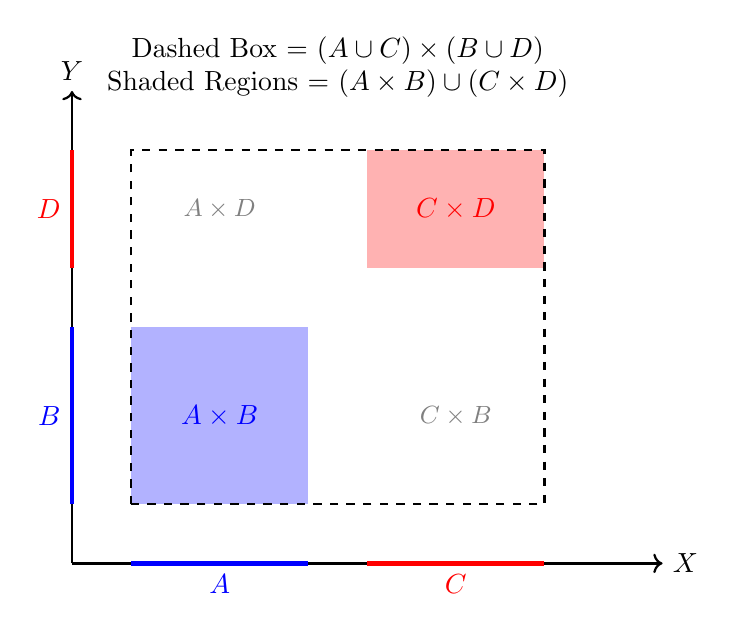
\begin{tikzpicture}[scale=1.5]
    % Axes
    \draw[->, thick] (0,0) -- (5,0) node[right] {$X$};
    \draw[->, thick] (0,0) -- (0,4) node[above] {$Y$};

    % Sets A, C on X-axis
    \draw[ultra thick, blue] (0.5, 0) -- (2, 0) node[midway, below] {$A$};
    \draw[ultra thick, red] (2.5, 0) -- (4, 0) node[midway, below] {$C$};

    % Sets B, D on Y-axis
    \draw[ultra thick, blue] (0, 0.5) -- (0, 2) node[midway, left] {$B$};
    \draw[ultra thick, red] (0, 2.5) -- (0, 3.5) node[midway, left] {$D$};

    % A x B
    \fill[blue, opacity=0.3] (0.5, 0.5) rectangle (2, 2);
    \node[blue] at (1.25, 1.25) {$A \times B$};

    % C x D
    \fill[red, opacity=0.3] (2.5, 2.5) rectangle (4, 3.5);
    \node[red] at (3.25, 3) {$C \times D$};

    % Bounding Box for (A U C) x (B U D)
    \draw[dashed, thick, black] (0.5, 0.5) rectangle (4, 3.5);
    \node[black, align=center] at (2.25, 4.2) {Dashed Box = $(A \cup C) \times (B \cup D)$ \\ Shaded Regions = $(A \times B) \cup (C \times D)$};
    
    % Cross terms
    \node[gray, font=\small] at (3.25, 1.25) {$C \times B$};
    \node[gray, font=\small] at (1.25, 3) {$A \times D$};

\end{tikzpicture}
\end{center}

\subsection{Heuristics \& "Cheats"}
\begin{itemize}
    \item \textbf{The "Empty Set Check":} Whenever a theorem involves $A \times B \subseteq C \times D \implies A \subseteq C$, immediately check if $A$ or $B$ being empty breaks the implication. It almost always does.
    \item \textbf{Dimensionality Check:} Never mix 1D elements with 2D pairs. If you write $x \in A \times B$, you have made a type error. It must be $(x, y) \in A \times B$.
\end{itemize}

\subsection{Pitfalls \& Fallacies}
\begin{itemize}
    \item \textbf{False Union Equality:} Assuming $(A \times B) \cup (C \times D) = (A \cup C) \times (B \cup D)$. As shown in the diagram above, this is a classic fallacy.
    \item \textbf{Power Set Cardinality Trap:} Assuming $\powerset(A \times B) = \powerset(A) \times \powerset(B)$. The left side is a set of sets of ordered pairs. The right side is a set of ordered pairs of sets. They are fundamentally different mathematical objects.
\end{itemize}

% ==========================================
% PART 5: Conceptual Synthesis
% ==========================================
\section{Part 5: Conceptual Synthesis and The "Big Picture"}

\subsection{A) Thematic Connections}
The core theme of this chapter is \textbf{dimensional synthesis}. We are learning how to rigorously define and manipulate multi-dimensional spaces using 1D logical axioms. This unifies previous topics (basic set operations, propositional logic) by showing that the algebraic structure of logic ($\land, \lor$) perfectly maps onto the geometric structure of Cartesian spaces ($\cap, \cup$).

\subsection{B) Forward and Backward Links}
\begin{itemize}
    \item \textbf{Backward Links:} This topic relies heavily on the Kuratowski definition of ordered pairs from foundational set theory and the logical equivalences (De Morgan's) established in Chapter 2.
    \item \textbf{Forward Links:} Cartesian products are the absolute bedrock for all advanced mathematics. A \textit{relation} is defined strictly as a subset of $A \times B$. A \textit{function} is a specific type of relation. In topology, the product topology on $X \times Y$ is built using Cartesian products of open sets. In measure theory, understanding $\sigma$-algebras on Cartesian products is the prerequisite for Fubini's Theorem (swapping the order of integration) and defining joint probability distributions.
\end{itemize}

% ==========================================
% PART 6: Abstract Real-World Modeling
% ==========================================
\section{Part 6: Abstract Real-World Modeling (AI, ML, \& Quant Finance)}

\subsection{A) Concrete Scenarios}
\begin{enumerate}
    \item \textbf{Joint Probability Spaces in Machine Learning:} In Bayesian Networks and Generative AI, we rarely deal with a single random variable. If $X$ is the space of image pixels and $Y$ is the space of text captions, the generative model learns a joint probability measure $\mathbb{P}$ over the Cartesian product space $\Omega = X \times Y$.
    \item \textbf{State-Action Spaces in Reinforcement Learning:} In Algorithmic Trading via Reinforcement Learning, an agent observes a market state $s \in S$ and takes an action $a \in A$. The reward function and transition dynamics are strictly defined over the Cartesian product $S \times A$.
\end{enumerate}

\subsection{B) Model Problem Setup: Markov Decision Process in Algorithmic Trading}
Let us rigorously model a Reinforcement Learning environment for high-frequency trading using Cartesian products.

\textbf{1. State Space ($S$):} Let $S = P \times V \times I$, where:
\begin{itemize}
    \item $P \subset \R^+$ is the set of possible asset prices.
    \item $V \subset \R^+$ is the set of possible order book volumes.
    \item $I \subset \Z$ is the set of possible inventory levels (number of shares held).
\end{itemize}
Thus, a single state is an ordered triplet $s = (p, v, i) \in S$.

\textbf{2. Action Space ($A$):} Let $A = \{-1, 0, 1\}$ representing Sell, Hold, and Buy.

\textbf{3. The Cartesian Product Space ($S \times A$):}
The core of the Markov Decision Process (MDP) operates on the Cartesian product $S \times A$. Every element $(s, a) \in S \times A$ represents a specific market condition paired with a specific trading decision.

\textbf{4. Transition Probability Measure:}
We define a transition kernel $P: (S \times A) \times \mathscr{B}(S) \to [0, 1]$, where $\mathscr{B}(S)$ is the Borel $\sigma$-algebra on $S$. For a given state-action pair $(s, a) \in S \times A$, $P((s, a), \cdot)$ yields a probability distribution over the next state $s'$.

\textbf{5. Optimization Problem (Bellman Equation):}
The quantitative researcher seeks to find an optimal policy $\pi: S \to A$ that maximizes the expected cumulative reward. The optimal action-value function $Q^*: S \times A \to \R$ is defined recursively over the Cartesian product space:
\[ Q^*(s, a) = \mathbb{E} \left[ R(s, a) + \gamma \max_{a' \in A} Q^*(s', a') \right] \]
Without the rigorous formalization of the Cartesian product $S \times A$, the domain of the $Q$-function and the transition kernel would be mathematically undefined, rendering the stochastic calculus of the Bellman equation impossible to prove or compute.

% ==========================================
% PART 7: Common Variations and Untested Concepts
% ==========================================
\section{Part 7: Common Variations and Untested Concepts}

A critical concept often introduced in advanced courses, but missing from this specific homework section, is the \textbf{Infinite Cartesian Product and the Axiom of Choice}.

\begin{definition}[Infinite Cartesian Product]
Let $I$ be an index set, and let $\{A_i\}_{i \in I}$ be a family of sets. The Cartesian product $\prod_{i \in I} A_i$ is defined as the set of all functions $f: I \to \bigcup_{i \in I} A_i$ such that $f(i) \in A_i$ for all $i \in I$.
\end{definition}

\begin{theorem}[Axiom of Choice Equivalence]
If $A_i \neq \emptyset$ for all $i \in I$, then $\prod_{i \in I} A_i \neq \emptyset$.
\end{theorem}

\begin{proof}[Proof of the Contrapositive (Without Axiom of Choice)]
We can easily prove the converse without the Axiom of Choice: If $\prod_{i \in I} A_i \neq \emptyset$, then $A_i \neq \emptyset$ for all $i \in I$.
Assume $\prod_{i \in I} A_i \neq \emptyset$. Then there exists at least one element $f \in \prod_{i \in I} A_i$. 
By definition, $f$ is a function such that $f(i) \in A_i$ for every $i \in I$. 
Since the function maps every index $i$ to some element in $A_i$, it must be that no $A_i$ is empty (if some $A_k = \emptyset$, $f(k)$ would be undefined, contradicting the existence of $f$). 
Thus, $A_i \neq \emptyset$ for all $i \in I$.
\end{proof}
\textit{Note:} Proving the forward direction requires the Axiom of Choice, a profound realization that bridges basic set theory with the foundations of modern mathematics.

% ==========================================
% PART 8: Advanced Diagnostic Testing
% ==========================================
\section{Part 8: Advanced Diagnostic Testing: "Find the Flaw"}

Below are five proofs that contain a subtle, critical logical flaw. Your task as the grader is to find the error.

\begin{flawprob}
\textbf{Claim:} For any sets $A, B, C, D$, $(A \cup B) \times (C \cup D) = (A \times C) \cup (B \times D)$. \\
\textbf{Proof:} Let $(x, y) \in (A \cup B) \times (C \cup D)$. By definition, $x \in A \cup B$ and $y \in C \cup D$. This means $(x \in A \lor x \in B)$ and $(y \in C \lor y \in D)$. Distributing the logical statements, we get $(x \in A \land y \in C) \lor (x \in B \land y \in D)$. Therefore, $(x, y) \in (A \times C) \cup (B \times D)$. The reverse inclusion follows similarly. $\blacksquare$
\end{flawprob}

\begin{flawprob}
\textbf{Claim:} If $A \times B = B \times A$, then $A = B$. \\
\textbf{Proof:} Assume $A \times B = B \times A$. Let $x \in A$. Choose some $y \in B$. Then the ordered pair $(x, y) \in A \times B$. Since $A \times B = B \times A$, it follows that $(x, y) \in B \times A$. By definition of the Cartesian product, the first coordinate must belong to the first set, so $x \in B$. Thus $A \subseteq B$. By a symmetric argument, $B \subseteq A$. Therefore, $A = B$. $\blacksquare$
\end{flawprob}

\begin{flawprob}
\textbf{Claim:} $(A \times B)^c = A^c \times B^c$, where $S^c$ denotes the complement of $S$ in a universal set $U$. \\
\textbf{Proof:} Let $(x, y) \in (A \times B)^c$. By definition of complement, $(x, y) \notin A \times B$. This means it is not the case that $(x \in A \land y \in B)$. By De Morgan's Law, $x \notin A \lor y \notin B$. This implies $x \in A^c \lor y \in B^c$. Therefore, $(x, y) \in A^c \times B^c$. $\blacksquare$
\end{flawprob}

\begin{flawprob}
\textbf{Claim:} $A \times (B \setminus C) = (A \times B) \setminus C$. \\
\textbf{Proof:} Let $(x, y) \in A \times (B \setminus C)$. Then $x \in A$ and $y \in B \setminus C$. This means $y \in B$ and $y \notin C$. Since $x \in A$ and $y \in B$, we have $(x, y) \in A \times B$. Since $y \notin C$, the pair $(x, y)$ cannot be in $C$. Therefore, $(x, y) \in (A \times B) \setminus C$. $\blacksquare$
\end{flawprob}

\begin{flawprob}
\textbf{Claim:} $\powerset(A \times B) = \powerset(A) \times \powerset(B)$. \\
\textbf{Proof:} Let $S \in \powerset(A \times B)$. Then $S \subseteq A \times B$. This means every element in $S$ is an ordered pair $(x, y)$ where $x \in A$ and $y \in B$. We can project $S$ into two sets: $S_A \subseteq A$ and $S_B \subseteq B$. Since $S_A \in \powerset(A)$ and $S_B \in \powerset(B)$, the pair $(S_A, S_B) \in \powerset(A) \times \powerset(B)$. Thus the sets are equal. $\blacksquare$
\end{flawprob}

\newpage
\subsection{Solution Key for Diagnostic Testing}

\textbf{Resolution to Problem 1:}
\textit{Flaw:} The logical distribution step is false. $(P \lor Q) \land (R \lor S)$ is NOT logically equivalent to $(P \land R) \lor (Q \land S)$. It actually expands to $(P \land R) \lor (P \land S) \lor (Q \land R) \lor (Q \land S)$. 
\textit{Correction:} The correct expansion yields $(A \times C) \cup (A \times D) \cup (B \times C) \cup (B \times D)$.

\textbf{Resolution to Problem 2:}
\textit{Flaw:} The proof assumes we can "Choose some $y \in B$". If $B = \emptyset$, we cannot choose such a $y$, and the proof collapses. (e.g., $\{1\} \times \emptyset = \emptyset \times \{1\} = \emptyset$, but $\{1\} \neq \emptyset$).
\textit{Correction:} The claim is false unless we add the hypothesis that $A \neq \emptyset$ and $B \neq \emptyset$.

\textbf{Resolution to Problem 3:}
\textit{Flaw:} The step "$x \in A^c \lor y \in B^c \implies (x, y) \in A^c \times B^c$" is invalid. The Cartesian product requires an AND ($\land$) relationship, not an OR ($\lor$). 
\textit{Correction:} The correct complement is $(A \times B)^c = (A^c \times U) \cup (U \times B^c)$.

\textbf{Resolution to Problem 4:}
\textit{Flaw:} Type mismatch. The expression $(A \times B) \setminus C$ is mathematically nonsensical if $C$ is a 1D set, because you are subtracting 1D elements from 2D ordered pairs. 
\textit{Correction:} The correct theorem is $A \times (B \setminus C) = (A \times B) \setminus (A \times C)$.

\textbf{Resolution to Problem 5:}
\textit{Flaw:} The proof conflates a subset of pairs with a pair of subsets. $S \in \powerset(A \times B)$ is a set of ordered pairs. $(S_A, S_B) \in \powerset(A) \times \powerset(B)$ is a single ordered pair containing two sets. They are entirely different data structures.
\textit{Correction:} The claim is fundamentally false. As shown in Exercise 4.61, they don't even have the same cardinality.

\end{document}